\documentclass[12pt,a4paper]{article}
\usepackage[a4paper,margin=2.5cm]{geometry}
\usepackage{fontspec}
\usepackage[vietnamese]{babel}
\usepackage{graphicx}
\usepackage{booktabs}
\usepackage{array}
\usepackage{float}
\usepackage{hyperref}
\usepackage{enumitem}
\usepackage{setspace}
\usepackage{titlesec}
\usepackage{longtable}
\usepackage{xcolor}

\setmainfont{Times New Roman}
\setstretch{1.25}
\hypersetup{
    colorlinks=true,
    linkcolor=blue,
    urlcolor=blue
}
\titleformat{\section}{\large\bfseries}{\thesection.}{0.5em}{}
\titleformat{\subsection}{\normalsize\bfseries}{\thesubsection.}{0.5em}{}

\begin{document}

\begin{titlepage}
    \centering
    {\large ĐẠI HỌC HUẾ \\[0.3cm]}
    {\large BÁO CÁO CUỐI HỌC PHẦN \\[0.8cm]}
    {\Large \textbf{LỌC BÌNH LUẬN ĐỘC HẠI VÀ QUẢNG CÁO RÁC CHO FANPAGE LỚN} \\[1.0cm]}

    \begin{tabular}{>{\bfseries}p{4.2cm}p{9cm}}
        Họ và tên sinh viên: & Đặng Tấn Phát \\
        Mã sinh viên: & 22T1020307 \\
        Học phần: & Khai phá dữ liệu / Máy học ứng dụng \\
        Hình thức nộp: & PDF sinh từ \LaTeX \\
    \end{tabular}

    \vfill

    {\large Ngày hoàn thành: 06/04/2026}
\end{titlepage}

\section{Xác lập bài toán}

\subsection{Bối cảnh thực tế}
Fanpage lớn thường nhận số lượng bình luận rất lớn trong thời gian ngắn. Trong đó có hai nhóm gây ảnh hưởng trực tiếp đến chất lượng vận hành:
\begin{itemize}[leftmargin=1.2cm]
    \item bình luận độc hại: chửi bới, xúc phạm, công kích người khác;
    \item bình luận quảng cáo rác: chèn số điện thoại, lời mời inbox, bán hàng, tuyển cộng tác viên hoặc điều hướng sang nền tảng khác.
\end{itemize}

Nếu kiểm duyệt hoàn toàn bằng tay, quản trị viên sẽ gặp ba vấn đề chính: tốn thời gian, phản ứng chậm và khó giữ trải nghiệm tương tác lành mạnh. Vì vậy đề tài hướng đến một hệ thống hỗ trợ kiểm duyệt có thể sàng lọc nhanh những trường hợp rõ ràng, đồng thời chuyển các trường hợp chưa chắc chắn sang bước kiểm tra thủ công.

\subsection{Đối tượng dữ liệu}
Đề tài sử dụng bộ dữ liệu tiếng Việt \textbf{ViCTSD} cho bài toán phát hiện bình luận độc hại. Đây là lựa chọn phù hợp vì dữ liệu bám sát ngữ cảnh bình luận mạng xã hội tiếng Việt thay vì văn bản chuẩn hóa.

Quy mô dữ liệu sử dụng trong source code hiện tại:
\begin{itemize}[leftmargin=1.2cm]
    \item tập huấn luyện: 7{,}000 bình luận, tỷ lệ toxic 10.84\%;
    \item tập validation: 2{,}000 bình luận, tỷ lệ toxic 11.60\%;
    \item tập kiểm thử: 1{,}000 bình luận, tỷ lệ toxic 11.00\%.
\end{itemize}

Điểm đáng chú ý là dữ liệu bị lệch lớp khá rõ, vì nhóm toxic chỉ chiếm khoảng 11\%. Điều này ảnh hưởng trực tiếp đến cách chọn mô hình và cách diễn giải metrics.

\subsection{Mục tiêu và giá trị mang lại}
Mục tiêu của đề tài không phải thay thế hoàn toàn con người, mà là tạo ra một cơ chế \textbf{lọc trước} để giảm tải vận hành. Giá trị thực tế của hệ thống nằm ở ba điểm:
\begin{itemize}[leftmargin=1.2cm]
    \item tự động ẩn các bình luận spam rõ ràng;
    \item phát hiện sớm bình luận toxic để cảnh báo hoặc chuyển kiểm duyệt;
    \item cung cấp giao diện web để người dùng không chuyên vẫn có thể quan sát dữ liệu, chạy dự đoán và xem hiệu năng mô hình.
\end{itemize}

Vì vậy, lời giải được thiết kế theo hướng \textbf{đủ đơn giản để triển khai}, \textbf{dễ giải thích}, nhưng vẫn phản ánh đúng bài toán thực tế.

\section{Tiền xử lý và đặc trưng}

\subsection{Lý do phải tiền xử lý}
Văn bản bình luận trên mạng xã hội thường có nhiều nhiễu: viết hoa viết thường không đồng nhất, kéo dài ký tự, chèn link, email, số điện thoại hoặc nhắc đến người dùng. Nếu giữ nguyên dữ liệu thô, số lượng biến thể bề mặt tăng rất nhanh, làm mô hình học máy tuyến tính khó học được mẫu ổn định.

Vì vậy, bước tiền xử lý trong mã nguồn được xây dựng để \textbf{giảm độ phân mảnh của từ vựng} nhưng vẫn giữ lại tín hiệu hữu ích cho phân loại.

\subsection{Các thao tác làm sạch dữ liệu}
Trong source code, văn bản được chuẩn hóa theo các nguyên tắc sau:
\begin{itemize}[leftmargin=1.2cm]
    \item chuyển về chữ thường để giảm biến thể cùng nghĩa;
    \item chuẩn hóa khoảng trắng;
    \item thay đường dẫn web bằng token \texttt{<url>};
    \item thay email bằng token \texttt{<email>};
    \item thay nhắc người dùng bằng token \texttt{<user>};
    \item thay các chuỗi số dài bằng token \texttt{<number>};
    \item rút gọn ký tự lặp bất thường để giảm nhiễu kiểu ``nguuuuu'' hoặc ``hayyyyy''.
\end{itemize}

Lý do chọn cách làm này là để mô hình không phải học riêng từng biến thể hiển thị, mà học theo \textbf{mẫu hành vi ngôn ngữ}. Ví dụ, nhiều kiểu link khác nhau đều được gom về một tín hiệu chung là \texttt{<url>}, giúp việc nhận diện spam ổn định hơn.

\subsection{Biểu diễn đặc trưng}
Đề tài sử dụng \textbf{TF-IDF} để biến đổi văn bản sang vector đặc trưng. Cấu hình hiện tại trong mã huấn luyện là:
\begin{itemize}[leftmargin=1.2cm]
    \item \texttt{ngram\_range=(1, 2)};
    \item \texttt{min\_df=3};
    \item \texttt{max\_features=30000};
    \item \texttt{sublinear\_tf=True}.
\end{itemize}

Việc chọn TF-IDF thay vì đặc trưng đơn giản như Bag-of-Words có hai lý do:
\begin{itemize}[leftmargin=1.2cm]
    \item TF-IDF giảm trọng số của các từ quá phổ biến nên mô hình chú ý nhiều hơn đến các từ hoặc cụm từ mang tính phân biệt;
    \item n-gram mức 1--2 giúp giữ được một phần ngữ cảnh cục bộ như ``mất dạy'', ``liên hệ'', ``giảm giá'', vốn quan trọng cho cả toxic và spam.
\end{itemize}

\subsection{Vì sao còn dùng rule-based cho spam}
Spam trên mạng xã hội thường có các tín hiệu cấu trúc rất rõ như link, số điện thoại hoặc cụm từ chào bán. Với loại mẫu này, một luật đơn giản thường hiệu quả và ổn định hơn so với việc ép mô hình văn bản học toàn bộ. Do đó hệ thống được thiết kế theo hướng kết hợp:
\begin{itemize}[leftmargin=1.2cm]
    \item tầng 1: rule-based để bắt spam rõ ràng;
    \item tầng 2: mô hình học máy để chấm điểm toxic cho phần còn lại.
\end{itemize}

Lựa chọn này giúp tiết kiệm tài nguyên huấn luyện và làm cho quyết định cuối cùng dễ giải thích hơn trong báo cáo.

\section{Thực thi mô hình}

\subsection{Lý do chọn Linear Regression}
Phiên bản hiện tại của đề tài chỉ sử dụng \textbf{một mô hình duy nhất là Linear Regression}. Đây không phải là lựa chọn mạnh nhất về mặt ngữ nghĩa, nhưng phù hợp với mục tiêu học phần ở ba điểm:
\begin{itemize}[leftmargin=1.2cm]
    \item dễ huấn luyện, nhanh, ít phụ thuộc thư viện nặng;
    \item dễ giải thích mối liên hệ giữa đặc trưng TF-IDF và đầu ra dự đoán;
    \item dễ đồng bộ giữa notebook, source code và web app.
\end{itemize}

Thay vì dự đoán trực tiếp nhãn rời rạc, mô hình sinh ra một \textbf{điểm toxic liên tục}. Điểm này được chặn về đoạn $[0, 1]$, sau đó dùng ngưỡng để chuyển sang nhãn \texttt{clean}/\texttt{toxic}. Cách làm này phù hợp với hệ thống kiểm duyệt vì:
\begin{itemize}[leftmargin=1.2cm]
    \item có thể điều chỉnh ngưỡng theo nhu cầu vận hành;
    \item dễ xây dựng vùng chuyển kiểm duyệt thủ công;
    \item thuận tiện cho giao diện web hiển thị mức độ rủi ro thay vì chỉ hiển thị nhãn cứng.
\end{itemize}

\subsection{Quy trình huấn luyện}
Quy trình huấn luyện hiện tại được triển khai trong file \texttt{train\_linear\_regression.py} theo thứ tự:
\begin{enumerate}[leftmargin=1.2cm]
    \item đọc dữ liệu train, validation, test;
    \item gộp train và validation để tăng lượng dữ liệu học;
    \item xây dựng pipeline \texttt{TF-IDF + LinearRegression};
    \item huấn luyện trên tập train+validation;
    \item dự đoán trên tập test;
    \item chặn đầu ra về $[0,1]$ và dùng ngưỡng 0.5 để phân lớp;
    \item lưu model, metrics, predictions, errors và confusion matrix.
\end{enumerate}

Lý do gộp train và validation trong phiên bản cuối là vì bài toán đang dùng một mô hình đơn giản và mục tiêu chính là tạo ra artifact nhất quán cho web app. Cách này giúp mô hình tận dụng tối đa dữ liệu sẵn có trước khi đánh giá trên tập test độc lập.

\subsection{Quy trình triển khai trong web app}
Trong web app Streamlit, luồng xử lý một bình luận được thiết kế theo logic nghiệp vụ:
\begin{enumerate}[leftmargin=1.2cm]
    \item người dùng nhập bình luận;
    \item hệ thống kiểm tra spam bằng tập luật;
    \item nếu spam score đủ cao thì ưu tiên xử lý như spam;
    \item nếu không phải spam rõ ràng thì mô hình Linear Regression chấm điểm toxic;
    \item dựa trên điểm toxic và ngưỡng giao diện, hệ thống đưa ra một trong ba quyết định: giữ bình luận, chuyển kiểm duyệt thủ công hoặc ẩn tự động.
\end{enumerate}

Điểm mạnh của cách triển khai này là \textbf{quyết định cuối cùng không phụ thuộc hoàn toàn vào mô hình}. Đó là lựa chọn phù hợp cho một hệ thống hỗ trợ kiểm duyệt trong thực tế.

\section{Phân tích và đánh giá}

\subsection{Kết quả định lượng}
Trên tập test 1{,}000 mẫu, mô hình hiện tại cho kết quả như Bảng~\ref{tab:metrics}.

\begin{table}[H]
    \centering
    \caption{Các chỉ số đánh giá của mô hình Linear Regression}
    \label{tab:metrics}
    \begin{tabular}{l c}
        \toprule
        Chỉ số & Giá trị \\
        \midrule
        Accuracy & 0.8740 \\
        Precision (toxic) & 0.4216 \\
        Recall (toxic) & 0.3909 \\
        F1-score (toxic) & 0.4057 \\
        Ngưỡng phân lớp & 0.50 \\
        \bottomrule
    \end{tabular}
\end{table}

Confusion matrix tương ứng:
\begin{itemize}[leftmargin=1.2cm]
    \item True Negative: 831
    \item False Positive: 59
    \item False Negative: 67
    \item True Positive: 43
\end{itemize}

\begin{figure}[H]
    \centering
    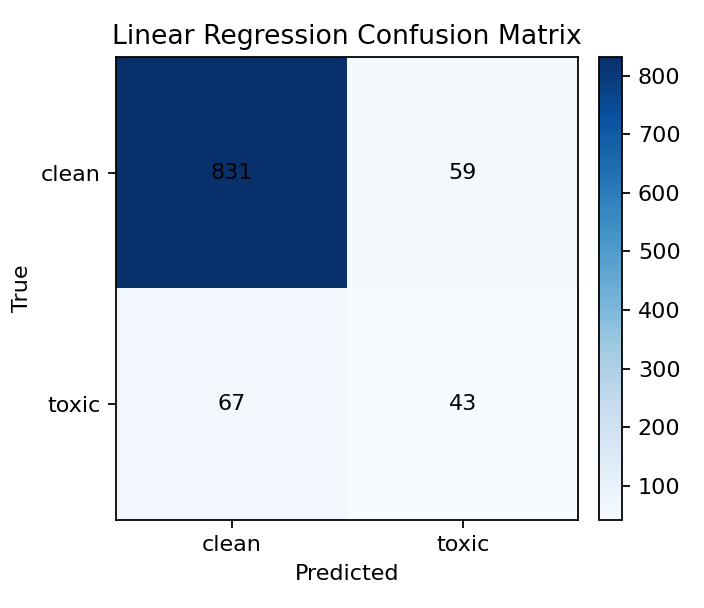
\includegraphics[width=0.58\textwidth]{reports/linear_regression_confusion_matrix.png}
    \caption{Confusion matrix của mô hình Linear Regression}
\end{figure}

\subsection{Diễn giải kết quả}
Kết quả cho thấy độ chính xác tổng thể khá cao, nhưng chỉ số trên lớp toxic còn hạn chế. Đây là hiện tượng hợp lý chứ không phải bất thường, vì:
\begin{itemize}[leftmargin=1.2cm]
    \item dữ liệu bị lệch lớp nên mô hình dễ thiên về lớp clean;
    \item Linear Regression là mô hình tuyến tính, mạnh ở việc khai thác từ khóa và mẫu cục bộ nhưng yếu ở ngữ cảnh sâu;
    \item một phần toxic xuất hiện dưới dạng mỉa mai, châm biếm hoặc công kích gián tiếp nên không có tín hiệu từ vựng quá rõ.
\end{itemize}

Nói cách khác, mô hình hiện tại phù hợp để làm \textbf{bộ lọc nền} hoặc \textbf{bộ chấm điểm sơ bộ}, nhưng chưa đủ mạnh để coi là bộ phân xử cuối cùng cho mọi bình luận độc hại.

\subsection{Những gì mô hình làm tốt}
\begin{itemize}[leftmargin=1.2cm]
    \item phát hiện tốt các bình luận clean nên giúp hạn chế chặn nhầm diện rộng;
    \item bắt được các toxic có dấu hiệu từ ngữ rõ ràng;
    \item tích hợp tốt với luật spam để tạo thành quy trình kiểm duyệt hai tầng;
    \item chạy nhanh, phù hợp với web app cần phản hồi gần thời gian thực.
\end{itemize}

\subsection{Hạn chế của giải pháp}
Hạn chế chính của hệ thống nằm ở phần bình luận \textbf{mỉa mai, nói giảm nói tránh, châm biếm hoặc công kích gián tiếp}. Đây là nhóm trường hợp mà mô hình dễ dự đoán sai vì không thật sự hiểu ngữ nghĩa toàn câu.

Ngoài ra, rule-based spam vẫn có thể bỏ sót các trường hợp người dùng cố ý viết biến thể để né luật, ví dụ thay ký tự, viết rời số điện thoại hoặc dùng câu quảng cáo ít từ khóa hơn.

\subsection{Hướng cải thiện}
Nếu tiếp tục phát triển, ba hướng cải thiện có giá trị nhất là:
\begin{itemize}[leftmargin=1.2cm]
    \item bổ sung dữ liệu toxic khó, đặc biệt là mỉa mai và công kích gián tiếp;
    \item mở rộng đặc trưng với n-gram dài hơn hoặc đặc trưng ký tự để bắt biến thể ngôn ngữ mạng;
    \item đưa vùng điểm trung gian vào quy trình kiểm duyệt thủ công thay vì ép mô hình quyết định cứng.
\end{itemize}

Điểm quan trọng là mọi cải tiến nên tiếp tục giữ tiêu chí nhất quán giữa \textbf{source code}, \textbf{artifact đánh giá} và \textbf{web app}, vì đây là yêu cầu cốt lõi của sản phẩm cuối kỳ.

\section{Kết luận}
Đề tài đã xây dựng được một hệ thống lọc bình luận có tính ứng dụng thực tế cho Fanpage lớn, gồm hai thành phần bổ trợ nhau: rule-based spam detection và mô hình Linear Regression cho toxic comment. Điểm mạnh của lời giải là đơn giản, dễ triển khai, dễ giải thích và đồng bộ tốt với giao diện web.

Tuy nhiên, kết quả đánh giá cũng chỉ ra rõ ràng rằng mô hình tuyến tính chưa đủ để xử lý trọn vẹn các trường hợp mang tính ngữ cảnh sâu như mỉa mai hoặc châm biếm. Vì vậy, giá trị chính của hệ thống hiện tại nằm ở vai trò \textbf{hỗ trợ kiểm duyệt} chứ chưa phải thay thế hoàn toàn con người.

\section*{Phụ lục: Tệp đồng bộ với báo cáo}
\begin{itemize}[leftmargin=1.2cm]
    \item Source code chính: \texttt{app.py}, \texttt{train\_linear\_regression.py}
    \item Model đang sử dụng: \texttt{models/linear\_regression\_toxic\_pipeline.joblib}
    \item Metrics: \texttt{reports/linear\_regression\_metrics.json}
    \item Predictions: \texttt{reports/linear\_regression\_predictions.csv}
    \item Error analysis: \texttt{reports/linear\_regression\_errors.csv}
    \item Web app local: \texttt{streamlit run app.py}
    \item URL triển khai:
    \texttt{[điền URL của web app nếu có public deployment]}
\end{itemize}

\end{document}
